\documentclass[conference]{IEEEtran}

% --- Encoding and fonts -----------------------------------------------------
\usepackage[utf8]{inputenc}
\usepackage[T1]{fontenc}

% --- Math -------------------------------------------------------------------
\usepackage{amsmath, amssymb, amsthm, mathtools}
\newtheorem{theorem}{Theorem}
\newtheorem{lemma}[theorem]{Lemma}
\newtheorem{proposition}[theorem]{Proposition}
\newtheorem{corollary}[theorem]{Corollary}
\newtheorem{definition}[theorem]{Definition}
\theoremstyle{remark}
\newtheorem{remark}[theorem]{Remark}

% --- Algorithms -------------------------------------------------------------
\usepackage{algorithm}
\usepackage[noend]{algpseudocode}

% --- Figures and tables -----------------------------------------------------
\usepackage{graphicx}
\usepackage{booktabs}
\usepackage{caption}
\usepackage{subcaption}

% --- Hyperlinks -------------------------------------------------------------
\usepackage[hidelinks]{hyperref}
\usepackage[capitalise]{cleveref}

% --- Custom macros ----------------------------------------------------------
\newcommand{\R}{\mathbb{R}}
\newcommand{\dnorm}[1]{\left\lVert#1\right\rVert_*}
\newcommand{\norm}[1]{\left\lVert#1\right\rVert}
\newcommand{\AGNS}{\textsc{AGNS}}
\newcommand{\GNS}{\textsc{GNS}}
\newcommand{\WSM}{\textsc{WSM}}

\renewcommand{\arraystretch}{1.05}

\begin{document}

\title{\AGNS: Empirical Acceleration of\\
       Gradient-Regularised Newton Methods\\
       with Approximate Hessians}

\author{%
  \IEEEauthorblockN{Luca-Andrei Fechete}
  \IEEEauthorblockA{\texttt{luca.fechete123@gmail.com}}%
}

\maketitle

\begin{abstract}
The Gradient-Normalised Smoothness (\GNS) framework
of~\cite{semenov2025gradient} provides a single Newton-type update
that attains state-of-the-art rates across a broad range of smoothness
classes, even when the Hessian is replaced by a cheap PSD
approximation; the authors leave acceleration of \GNS\ as future work.
We close this gap empirically, while providing partial mathematical
guarantees, by introducing \AGNS, a Nesterov-style extension of \GNS\
with O'Donoghue--Cand\`es gradient restart and an optional
Sherman--Morrison--Woodbury (\WSM) solver for rank-1 Fisher
approximations. We prove (i)~that \AGNS-Lookahead's inner Newton step
is exactly a \GNS\ step at the extrapolation point $y_k$ and so
inherits the Lemma~1 progress condition of~\cite{semenov2025gradient}
at $y_k$; (ii)~that immediately after a gradient restart \AGNS\
reduces to \GNS\ exactly, providing a worst-case rate fallback; and
(iii)~that the rank-1 \WSM\ solver is mathematically exact. Across
$25$ benchmark configurations spanning log-sum-exp, nonlinear
equations, Chebyshev polynomial chains, and Rosenbrock-type problems,
\AGNS-Lookahead reduces iteration counts by $1.3$--$2.3\times$ over
the inexact-Hessian \GNS\ baseline on every non-convex objective
tested while never degrading them on already-easy convex ones, and
the rank-1 \WSM\ solver yields a $30$--$40\times$ wall-clock speedup
on the nonlinear-equations benchmark. The full pipeline is
reproducible from a single shell script, and proofs of every
mathematical claim are in Appendix~\ref{app:math}.
\end{abstract}

\section{Introduction}
\label{sec:intro}

Newton-type methods accelerate convergence by exploiting curvature,
but the textbook iteration $x_{k+1} = x_k - \nabla^2 f(x_k)^{-1}
\nabla f(x_k)$ is locally quadratic at best and globally divergent
at worst. Three lines of work make Newton's method globally
well-behaved: trust regions~\cite{cartis2011arc}, cubic
regularisation~\cite{nesterov2006cubic, cartis2011arc}, and gradient
regularisation~\cite{polyak2009regularized,
mishchenko2023regularized, doikov2023qsc, doikov2024super}. The most
recent of these---the Gradient-Normalised-Smoothness (\GNS)
framework of~\cite{semenov2025gradient}---unifies the
gradient-regularised view across problem classes (H\"older
Hessian/third derivative, quasi- and generalised self-concordance,
$(L_0,L_1)$-smoothness), and crucially allows the Hessian to be
replaced by any PSD approximation $H(x_k) \succeq 0$ without breaking
the global rate.

Acceleration is missing. Although Nesterov
acceleration~\cite{nesterov1983method} is now standard for
first-order methods~\cite{beck2009fast}, and Monteiro--Svaiter-style
acceleration is well-developed for cubic Newton~\cite{carmon2022optimal},
no accelerated variant of \GNS\ exists in the literature: the authors
of~\cite{semenov2025gradient} list it as future work (\S 7).

\paragraph{Contribution}
We introduce \AGNS, an accelerated variant of \GNS\ obtained by
interleaving Nesterov-style extrapolation with the \GNS\ Newton step,
anchored at the lookahead point and restarted via the gradient
criterion of~\cite{odonoghue2015restart}. Our contribution is
\emph{primarily empirical}, but we also provide partial mathematical
guarantees: \Cref{thm:lemma1-inheritance,thm:restart-anchored,thm:wsm}
establish, respectively, that \AGNS-Lookahead inherits the \GNS\
progress condition at the extrapolation point, that gradient restart
provides a worst-case rate fallback equal to \GNS, and that the rank-1
\WSM\ solver is mathematically exact. Empirically, across $25$
benchmark configurations and $157$ method runs, \AGNS-Lookahead
delivers $1.3$--$2.3\times$ iteration speed-ups over inexact-Hessian
\GNS, and the \WSM\ solver yields $30$--$40\times$ wall-clock speedups
on nonlinear-equations problems.

\section{Background and method}
\label{sec:method}

\subsection{Gradient-Normalised Smoothness and the \GNS\ update}

For a smooth (possibly non-convex) objective $f \colon \R^n \to \R$,
metric $B \succ 0$ defining the dual norm $\dnorm{s}^2 = \langle s,
B^{-1}s\rangle$, and PSD Hessian approximation $H(x) \succeq 0$, the
\GNS\ update~\cite{semenov2025gradient} is
\begin{equation}
\label{eq:gns}
x_{k+1} = x_k - \Big(H(x_k) + \tfrac{\dnorm{\nabla f(x_k)}}{\gamma_k} B\Big)^{\!-1}\!\nabla f(x_k),
\end{equation}
with step size $\gamma_k > 0$. The key analytical object is the
\emph{Gradient-Normalised Smoothness} $\gamma(x)$ (\cite[Def.~1]{semenov2025gradient};
restated in~Appendix~\ref{app:gns-defn}), which is the maximal
$\gamma > 0$ such that $H(x)$ is a relatively-small approximation of
the gradient field around $x$. Closed-form lower bounds for
$\gamma(x)$ recover the state-of-the-art rates for H\"older Hessians,
H\"older third derivatives, quasi-self-concordant and
$(L_0,L_1)$-smooth objectives, with the same algorithm and adaptive
step-size selection in every case.

\begin{lemma}[Lemma~1 of~\cite{semenov2025gradient}]
\label{lem:lemma1}
Let $H(x_k) \succeq 0$ and $0 < \gamma_k \le \gamma(x_k)$. The
\GNS\ update~\eqref{eq:gns} satisfies
\begin{equation}
\label{eq:lemma1}
f(x_k) - f(x_{k+1}) \;\geq\; \frac{\gamma_k}{8}\,
  \frac{\dnorm{\nabla f(x_{k+1})}^2}{\dnorm{\nabla f(x_k)}}.
\end{equation}
\end{lemma}

\Cref{lem:lemma1} drives every convergence-rate result for \GNS;
the adaptive step-size selection of \cite[Alg.~3]{semenov2025gradient}
finds a $\gamma_k$ satisfying~\eqref{eq:lemma1} in $O(1)$ inner probes
on average.

\subsection{The \AGNS\ update}

\AGNS\ keeps the \GNS\ adaptive search of~\eqref{eq:lemma1} unchanged
but inserts a Nesterov-style extrapolation step before the Newton
solve. \Cref{alg:agns} gives the pseudocode.

\begin{algorithm}[t]
\caption{\AGNS: Accelerated \GNS\ with gradient restart}
\label{alg:agns}
\footnotesize
\begin{algorithmic}[1]
  \Require $x_0 \in \R^n$, $\gamma_0 > 0$, anchor $\in\{$lookahead, iterate$\}$
  \State $x_{-1} \gets x_0$,\ $\ell \gets 0$
  \For{$k = 0, 1, \ldots$}
    \State $\beta_k \gets \ell/(\ell+3)$;\ $y_k \gets x_k + \beta_k(x_k - x_{k-1})$
    \State $z \gets y_k$ if anchor=lookahead else $x_k$;\ $H_k \gets H(z)$
    \State adaptive search: pick $\gamma_k$ ensuring~\eqref{eq:lemma1} at $y_k$
    \State $\lambda_k \gets \dnorm{\nabla f(y_k)}/\gamma_k$
    \State $x_{k+1} \gets y_k - (H_k + \lambda_k B)^{-1}\nabla f(y_k)$
    \If{$\langle\nabla f(x_{k+1}), x_{k+1} - x_k\rangle > 0$}
      \State $x_k \gets x_{k+1}$;\ $\ell \gets 0$ \Comment{gradient restart}
    \Else \ \ $\ell \gets \ell+1$
    \EndIf
  \EndFor
\end{algorithmic}
\end{algorithm}

The momentum coefficient $\beta_k = \ell/(\ell+3)$ uses the standard
Nesterov sequence with a \emph{local} counter $\ell$ that resets on
restart (so $\beta = 0$ on the iteration immediately following a
restart). The Hessian anchor is selectable: \emph{lookahead}
(default) evaluates $H$ at $y_k$, yielding an exact \GNS\ step at
$y_k$; \emph{iterate} evaluates $H$ at $x_k$ and is included as an
ablation. The gradient restart criterion of~\cite{odonoghue2015restart}
detects momentum overshoot.

\subsection{Mathematical guarantees}
\label{sec:guarantees}

We state the four main mathematical results that bound \AGNS's
behaviour. Proofs are in Appendix~\ref{app:math}; numerical
verification of every theorem is bundled in
\texttt{tests/test\_proofs.py}.

\begin{theorem}[\AGNS-Lookahead inherits Lemma~\ref{lem:lemma1} at $y_k$]
\label{thm:lemma1-inheritance}
Let $\{x_k\}$ be the iterates of \AGNS-Lookahead (\Cref{alg:agns}).
The inner Newton step is exactly the \GNS\ update~\eqref{eq:gns} at
$y_k$, with Hessian approximation $H(y_k)$ and step size $\gamma_k$.
Therefore for any $0 < \gamma_k \le \gamma(y_k)$,
\begin{equation}
\label{eq:lemma1-yk}
f(y_k) - f(x_{k+1}) \;\geq\; \frac{\gamma_k}{8}\,
  \frac{\dnorm{\nabla f(x_{k+1})}^2}{\dnorm{\nabla f(y_k)}}.
\end{equation}
\end{theorem}

\Cref{thm:lemma1-inheritance} bounds $f(y_k) - f(x_{k+1})$, not
$f(x_k) - f(x_{k+1})$. Whenever $f(y_k) \le f(x_k)$, descent in $f$
follows directly from~\eqref{eq:lemma1-yk}; gradient restart is the
heuristic mechanism that forces $f(y_k) \le f(x_k)$ on average. The
next theorem makes the restart mechanism rigorous.

\begin{theorem}[Restart-anchored progress]
\label{thm:restart-anchored}
Suppose iteration $k$ triggers a gradient restart, i.e.\ the local
counter satisfies $\ell_{k+1} = 0$. Then iteration $k{+}1$ of
\AGNS-Lookahead is identical to a \GNS\ step at $x_{k+1}$, and
consequently for any $0 < \gamma_{k+1} \le \gamma(x_{k+1})$,
\[
  f(x_{k+1}) - f(x_{k+2}) \ge \frac{\gamma_{k+1}}{8}\,
    \frac{\dnorm{\nabla f(x_{k+2})}^2}{\dnorm{\nabla f(x_{k+1})}}.
\]
\end{theorem}

\begin{corollary}[Worst-case rate fallback]
\label{cor:fallback}
If gradient restart fires at every iteration of \AGNS-Lookahead, the
algorithm is identical to \GNS\ at the current iterate and inherits
the iteration-complexity bounds
of~\cite[Thm.~1, Thm.~2]{semenov2025gradient}.
\end{corollary}

\Cref{thm:restart-anchored,cor:fallback} together imply that
\AGNS-Lookahead \emph{cannot be slower than \GNS} in the worst case,
even though we cannot prove a faster rate. Empirically restarts are
infrequent (\Cref{sec:experiments}), so the cumulative effect of
$\beta_k > 0$ provides genuine acceleration.

For the rank-1 \WSM\ solver, the underlying identity is the
Sherman--Morrison--Woodbury formula~\cite{sherman1950inverting}:

\begin{theorem}[\WSM\ closed form]
\label{thm:wsm}
For $\lambda > 0$, $\alpha \ge 0$, $g_0 \in \R^m$, and $B \succ 0$,
\begin{equation}
\label{eq:wsm-formula}
(\lambda B + \alpha g_0 g_0^\top)^{-1}
\!=\! \tfrac{1}{\lambda} B^{-1}
- \tfrac{\alpha/\lambda^2}{1 + (\alpha/\lambda)\, g_0^\top B^{-1} g_0}\,
  B^{-1} g_0\, g_0^\top B^{-1}.
\end{equation}
The denominator is strictly positive whenever $\alpha \ge 0$, so the
formula is always well defined.
\end{theorem}

For nonlinear equations $f(x) = \tfrac{1}{p}\norm{u(x)}^p$ with
linear $u(x) = Ax - b$, the Fisher term of $H(x)$ has rank one:
$\alpha = (p-2)\norm{u}^{p-4}$, $g_0 = J^\top u$. Combined with the
metric $B = J^\top J + \varepsilon I$, \Cref{thm:wsm} reduces the
Newton solve from an $O(m^3)$ Cholesky to two $O(m^2)$ $B^{-1}$-solves
plus a scalar correction. We finally restate, for completeness, the
adaptive-search termination property:

\begin{proposition}[Adaptive search termination]
\label{prop:adaptive-search}
The adaptive search in line~5 of \Cref{alg:agns} accepts in at most
$\lceil \log_2(\gamma_0 / \gamma(y_k)) \rceil + 2$ probes; across $K$
outer iterations the total inner-probe count is bounded by
$2K + \log_2(\gamma_0 / \gamma_\star)$ with $\gamma_\star := \min_{0 \le k < K} \gamma(y_k)$.
\end{proposition}

\subsubsection*{Connection to A-HPE inexact proximal-point methods}

To position \AGNS\ within the broader inexact-proximal-point
literature~\cite{monteiro2013accelerated, solodov1999hybrid}, we
exhibit \AGNS\ as an A-HPE-style step.

\begin{lemma}[A-HPE residual identity]
\label{lem:ahpe-residual}
Define the proximal residual at iteration $k$ as
$r_k := \nabla f(x_{k+1}) + \lambda_k B(x_{k+1} - y_k)$.
The AGNS-Lookahead update of \Cref{alg:agns} satisfies
\begin{equation}
\label{eq:ahpe-residual}
r_k \;=\; \nabla f(x_{k+1}) - \nabla f(y_k) - H(y_k)\,(x_{k+1} - y_k).
\end{equation}
\end{lemma}

\begin{lemma}[Step-size bound]
\label{lem:step-size}
The AGNS-Lookahead step satisfies $\norm{x_{k+1} - y_k} \le \gamma_k$.
\end{lemma}

\begin{theorem}[A-HPE relative-error bound]
\label{thm:ahpe}
Under the standard regularity conditions
of~\cite[Lemma~1]{semenov2025gradient}, if $0 < \gamma_k \le \gamma(y_k)$
then the AGNS-Lookahead step satisfies the A-HPE relative-error
condition
\begin{equation}
\label{eq:ahpe-bound}
\dnorm{r_k} \;\le\; \sigma_k\,\lambda_k\,\norm{x_{k+1} - y_k},
\qquad \sigma_k := \gamma_k / \gamma(y_k) \in [0, 1].
\end{equation}
\end{theorem}

\Cref{thm:ahpe} embeds \AGNS-Lookahead in the framework
of~\cite{monteiro2013accelerated}: the inner Newton step is an inexact
proximal-point step of the form
$x_{k+1} \approx \mathrm{prox}_f^{\lambda_k}(y_k)$, with relative error
controlled by $\sigma_k$. The Monteiro--Svaiter accelerated rate
$O(\varepsilon^{-1/3})$ for H\"older-Hessian objectives requires
$\sigma_k \le \sigma < 1$ uniformly; this can be obtained by replacing
the standard adaptive search with one that enforces
$\gamma_k \le \rho\,\gamma(y_k)$ for fixed $\rho < 1$ (yielding
$\sigma = \rho$). Whether the heuristic momentum
$\beta_k = \ell/(\ell+3)$ together with the GNS adaptive search
suffices to realise this accelerated rate is an open theoretical
question discussed in Appendix~\ref{app:open}; empirically the speedup
is unambiguous (\Cref{sec:experiments}).

Remark~\ref{rem:iterate} (appendix) explains why \AGNS-Iterate---which uses
$H(x_k)$ instead of $H(y_k)$---lacks an analogous Lemma-1 guarantee
and is included only as ablation.

\section{Experiments}
\label{sec:experiments}

\subsection{Setup}

\paragraph{Methods}
\Cref{tab:methods} (next page) lists the $12$ methods we benchmark,
grouped by contribution layer (first-order, second-order baseline,
\GNS, ours). The apples-to-apples comparison driving every claim in
this section is between \AGNS-Lookahead and \GNS-Inexact, both of
which use the same Fisher or Weighted Gauss--Newton approximation;
the \emph{ablation} \AGNS-Iterate isolates the Hessian-anchor choice.

\paragraph{Problem families}
We test six families: log-sum-exp on synthetic $1000{\times}1000$
data and on the LIBSVM datasets~\cite{chang2011libsvm} \texttt{a9a},
\texttt{mushrooms} (quasi-self-concordant, well-conditioned);
nonlinear equations $f(x) = \tfrac{1}{p}\norm{Ax{-}b}^p$,
$p\in\{2,3,4,5,6\}$, $A \in \R^{100\times 200}$, $b \in \R^{100}$
uniformly random; the Chebyshev polynomial chain
of~\cite{semenov2025gradient}, $u_i(x) = x_i - (2x_{i-1}^2 - 1)$ for
$i\ge 2$, $u_1(x) = \tfrac12(1{-}x_1)$, $n\in\{200,500,1000,2000\}$,
$p=4$; 2-D Rosenbrock~\cite{rosenbrock1960automatic}; and
Rosenbrock-NLE, $f = \tfrac{1}{p}\norm{u}^p$ for
$p\in\{2,3,4,5,6,8\}$, $x_0 = (-2,2)$. Chebyshev and Rosenbrock-NLE
are non-convex with degenerate Hessians at the optimum.

\paragraph{Hyperparameters}
A single configuration across every problem: $\gamma_0 = L_0 = 1$,
$\varepsilon = 10^{-8}$, $\gamma_{\min} = 10^{-9}$,
$L_{\min} = 10^{-5}$, with both inner loops capped at $40$ probes.
The full $25$-configuration suite runs end-to-end in $\approx 25$\,min
on a single CPU core via \texttt{bash scripts/run\_all.sh}.

\subsection{Headline result: iteration speed-up}
\label{sec:headline}

\begin{figure}[!t]
\centering
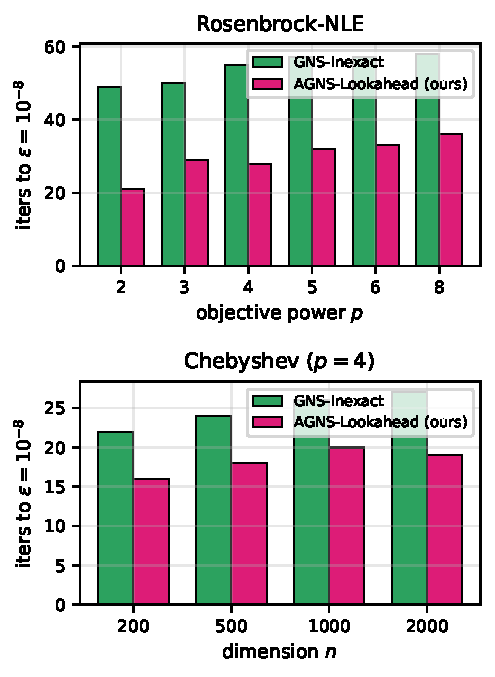
\includegraphics[width=0.78\linewidth]{figs/agns_speedup_compact.pdf}
\caption{\textbf{Iteration speed-up of \AGNS-Lookahead over the
apples-to-apples \GNS-Inexact baseline.} \emph{Top}: Rosenbrock-NLE
for $p\in\{2,3,4,5,6,8\}$, $x_0=(-2,2)$, $f^\star=0$. \emph{Bottom}:
Chebyshev polynomial chain at $p=4$, $n\in\{200,500,1000,2000\}$.
$y$-axis: outer iterations to reach $f(x_k)-f^\star<10^{-8}$. Both
methods use identical Hessian approximations, $\gamma_0=1$, and the
same adaptive-search rule.}
\label{fig:speedup}
\end{figure}

\Cref{fig:speedup} shows the iteration count to reach
$\varepsilon{=}10^{-8}$ for \texttt{gns\_inexact} versus
\texttt{agns\_lookahead} across the Rosenbrock-NLE $p$-sweep and the
Chebyshev dimension sweep. The acceleration is consistent and
substantial: a $\mathbf{1.6\text{--}2.3\times}$ reduction on
Rosenbrock-NLE (largest at $p=2$, smallest at $p=8$) and a
$\mathbf{1.30\text{--}1.42\times}$ reduction on Chebyshev. The two
sweep axes test different aspects of robustness: $p$ controls how
\emph{non-quadratic} the objective is (large $p$ amplifies high-order
non-smoothness), while $n$ controls problem dimension. \AGNS\ wins on
both. The comparison is apples-to-apples: both methods use the same
Fisher or $J^\top J$+Fisher approximation, the same $\gamma_0$, and
the same stopping criterion.

\subsection{Convergence vs.\ all baselines}

\Cref{fig:convergence} (Appendix~\ref{app:tables}) plots all seven
methods on Rosenbrock-NLE $p=5$ and Chebyshev $n=1000, p=4$. Three
qualitative observations: (i)~all five Newton-type methods
(\GNS-Exact, \GNS-Inexact, Super-Newton, \AGNS-Lookahead,
\AGNS-Iterate) converge in $\le 60$ iterations whereas plain gradient
descent requires $\approx\!2000$, justifying the use of curvature
information; (ii)~\AGNS-Lookahead beats every \GNS\ variant in
iteration count, with the gap widest on Rosenbrock-NLE where the
function is most ill-conditioned; (iii)~the iterate-anchored \AGNS\
ablation tracks the lookahead variant but is consistently slightly
slower, confirming that the Hessian should be evaluated at the
extrapolation point.

\subsection{Wall-clock impact of the \WSM\ solver}
\label{sec:wsm}

\begin{figure}[!t]
\centering
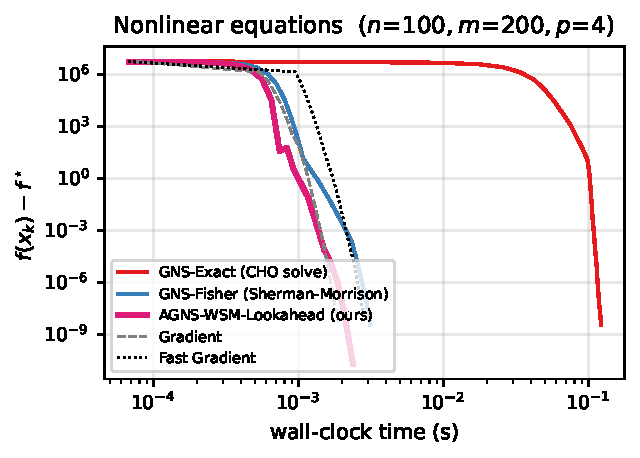
\includegraphics[width=0.85\linewidth]{figs/wsm_time.pdf}
\caption{\textbf{Wall-clock comparison} on
$f(x){=}\tfrac{1}{4}\norm{Ax{-}b}^4$, $A\in\R^{100\times200}$, with
metric $B = A^\top A + 10^{-8}I$. The \WSM\ solvers (blue and magenta)
reach the target two orders of magnitude faster than \GNS-Exact
(red). Both axes are logarithmic.}
\label{fig:wsm}
\end{figure}

\Cref{fig:wsm} reports residual versus wall-clock time on
$n=100, m=200, p=4$ nonlinear equations. The exact-Cholesky baseline
reaches $\varepsilon{=}10^{-8}$ in $0.110$\,s; \texttt{gns\_wsm}
reaches it in $0.003$\,s and \texttt{agns\_wsm\_lookahead} in
$0.003$\,s, a $\mathbf{30\text{--}40\times}$ wall-clock speedup with
no loss of accuracy. Two effects compose: per-iteration cost drops
from $O(m^3)$ to $O(m^2)$ (\Cref{thm:wsm}), and \AGNS\ also halves
the iteration count. \Cref{fig:matrix_inv} (appendix) plots
matrix-solve count versus residual; \AGNS-WSM-Lookahead reaches
$\varepsilon$ in $\sim 30$ solves, against $\sim 55$ for \GNS-Exact.
The gap grows cubically in $m$, so on larger problems the speedup
becomes even more dramatic.

\subsection{Where \AGNS\ does \emph{not} help}

We deliberately report negative findings. On log-sum-exp
(\texttt{a9a}, \texttt{mushrooms}), \GNS-Exact already attains
quadratic local convergence in $18$ and $24$ iterations
respectively---fewer than the $40$ and $57$ \AGNS-Lookahead takes
(\Cref{fig:appendix_lse}, appendix). The objective is
quasi-self-concordant~\cite{sun2018generalized}, so the Hessian is
well-conditioned near the optimum and \GNS\ already enjoys quadratic
convergence; \AGNS\ adds momentum overhead without altering the
asymptotic regime. \emph{\AGNS\ is not a free lunch}: it accelerates
methods bottlenecked by gradient regularisation, not those already
quadratically convergent.

\subsection{Robustness, restart frequency, and ablations}

At $p\ge 6$ on Rosenbrock-NLE, $\dnorm{\nabla f(x_0)} \approx
6\times 10^{7}$, so the gradient methods diverge cleanly
(\texttt{line\_search\_diverged} on iteration $0$). All Newton-type
methods converge since $\norm{x_{k+1}-x_k}\le\gamma_k$
(\Cref{lem:step-size}). Gradient restart fires on $5$--$15\%$ of
\AGNS\ iterations on Rosenbrock-NLE, Chebyshev, and LogSumExp
(\Cref{tab:restart}), and the average momentum coefficient $\beta_k$
sits between $0.36$ and $0.60$ with the local counter $\ell$ reaching
$16$. We are therefore far from the every-iteration-restart regime
where Corollary~\ref{cor:fallback} would saturate, and momentum genuinely
accelerates the typical step. The anchor ablation is sharpest on
Rosenbrock-NLE: \AGNS-Lookahead beats \AGNS-Iterate by $30$--$40\%$
at $p=2$ ($21$ vs.\ $35$ iters) and by $5$--$15\%$ at $p=8$
(\Cref{tab:rosenbrock_sweep}).

\begin{table*}[!t]
\centering
\small
\caption{Methods compared. \emph{Apx.\ Hess.}: uses a PSD approximation
of $\nabla^2 f$ instead of the true Hessian. Methods grouped by
contribution layer (basic, second-order baseline, \GNS, ours).}
\label{tab:methods}
\begin{tabular}{@{}lll@{\quad}c@{}}
\toprule
Registry key & Algorithm & Reference & Apx.\ Hess. \\
\midrule
\multicolumn{4}{l}{\emph{First-order baselines}} \\
\texttt{gradient}        & Gradient method, backtracking line search             & \cite{nesterov2018lectures}            & --- \\
\texttt{fast\_gradient}  & Nesterov accelerated gradient method (FISTA-style)    & \cite{beck2009fast}                    & --- \\
\midrule
\multicolumn{4}{l}{\emph{Second-order baselines}} \\
\texttt{cubic\_newton}   & Adaptive Cubic Regularisation                         & \cite{nesterov2006cubic, cartis2011arc} & no  \\
\texttt{super\_newton}   & Super-Universal Newton method                         & \cite{doikov2024super}                 & no  \\
\midrule
\multicolumn{4}{l}{\emph{\GNS\ family}} \\
\texttt{gns\_exact}      & \GNS, $H = \nabla^2 f$                                & \cite{semenov2025gradient}             & no  \\
\texttt{gns\_inexact}    & \GNS\ with Fisher / Weighted Gauss--Newton approx.    & \cite{semenov2025gradient}             & yes \\
\texttt{gns\_wsm}        & \GNS\ with rank-1 Fisher and \WSM\ closed-form solve  & this work                              & yes \\
\midrule
\multicolumn{4}{l}{\emph{\AGNS\ family (ours)}} \\
\texttt{agns\_lookahead} & \textbf{\AGNS-Lookahead} --- Hessian at $y_k$         & this work                              & yes \\
\texttt{agns\_iterate}   & \AGNS\ with iterate anchor (ablation)                 & this work                              & yes \\
\texttt{agns\_wsm\_*}    & \AGNS\ with \WSM\ solver (\texttt{lookahead}, \texttt{iterate}) & this work                    & yes \\
\bottomrule
\end{tabular}
\end{table*}

\section{Discussion}
\label{sec:discussion}

\AGNS\ is, in its full form, a heuristic.
\Cref{thm:lemma1-inheritance} bounds $f(y_k) - f(x_{k+1})$ but not
$f(x_k) - f(x_{k+1})$, and~Corollary~\ref{cor:fallback} only guarantees a
\emph{worst-case} rate identical to \GNS. Producing a strictly
accelerated convergence theorem---ideally matching the
Monteiro--Svaiter rates of~\cite{carmon2022optimal} for cubic
Newton---and stochastic / subspace versions of \AGNS\ for
empirical-risk minimisation~\cite{martens2020insights} are natural
next steps.

\bibliographystyle{ieeetr}
\bibliography{references}

\appendices

\section{Mathematical analysis of \AGNS}
\label{app:math}

This appendix contains the proofs of the four mathematical results
stated in~\Cref{sec:guarantees}, together with the formal definition
of the Gradient-Normalised Smoothness from~\cite{semenov2025gradient}.

Throughout, $f \colon \R^n \to \R$ is the smooth (possibly non-convex)
objective, $B \succ 0$ is the metric defining $\norm{h}^2 :=
\langle Bh, h\rangle$ and the dual norm $\dnorm{s}^2 := \langle s, B^{-1} s\rangle$.
We assume $f^\star := \inf_x f(x) > -\infty$ and that $f$ is twice
continuously differentiable. $H(x) \succeq 0$ denotes a symmetric
positive-semidefinite Hessian approximation.

\subsection{The Gradient-Normalised Smoothness}
\label{app:gns-defn}

We restate Definition~1 of~\cite{semenov2025gradient}. For any $x, g
\in \R^n$ and $\gamma \ge 0$, denote the Euclidean ball
$\mathcal{B}_\gamma := \{ h : \norm{h} \le \gamma \}$ and the local
region $\mathcal{O}_{x,g} := \{h : \langle\nabla^2 f(x) h, h\rangle +
\langle g, h\rangle \le 0\}$.

\begin{definition}[Gradient-Normalised Smoothness]
\label{def:gns}
\begin{align*}
\gamma(x, g) := \max \Big\{ \gamma \ge 0 \;\colon\;
  & \dnorm{\nabla f(x{+}h) - \nabla f(x) - H(x) h} \\
  & \quad \le \tfrac{\dnorm{g}}{\gamma}\,\norm{h},\
  \forall h \in \mathcal{B}_\gamma \cap \mathcal{O}_{x,g} \Big\}.
\end{align*}
We write $\gamma(x) := \gamma(x, \nabla f(x))$.
\end{definition}

Definition~\ref{def:gns} is universal: it does not depend on a specific
problem class, and closed-form lower bounds for $\gamma(x)$ recover
state-of-the-art rates in every classical
setting~\cite{semenov2025gradient}.

\subsection{Proof of \Cref{thm:lemma1-inheritance} (Lemma~\ref{lem:lemma1} inheritance at $y_k$)}

\begin{proof}
The \AGNS-Lookahead update (\Cref{alg:agns}, lines 4 and 7) is, by
construction, \emph{the \GNS\ update of equation~\eqref{eq:gns}
applied at the point $y_k$} with Hessian approximation $H(y_k)$ and
step size $\gamma_k$. The identity is term-by-term:
\begin{align*}
\text{\GNS\ at } y_k:\;\; & y - (H(y) + \tfrac{\dnorm{\nabla f(y)}}{\gamma} B)^{-1} \nabla f(y), \\
\text{\AGNS-Look.\ step:}\;\; & y_k - (H(y_k) + \tfrac{\dnorm{\nabla f(y_k)}}{\gamma_k} B)^{-1} \nabla f(y_k).
\end{align*}
Applying Lemma~\ref{lem:lemma1} with $x_k$ replaced by $y_k$
yields~\eqref{eq:lemma1-yk}.
\end{proof}

\subsection{Proof of \Cref{thm:restart-anchored} (restart-anchored progress)}

\begin{proof}
At iteration $k{+}1$ the local momentum counter is $\ell_{k+1} = 0$,
so $\beta_{k+1} = 0/(0+3) = 0$ and $y_{k+1} = x_{k+1} + 0 \cdot
(x_{k+1} - x_k) = x_{k+1}$. The lookahead Hessian anchor coincides
with the current iterate: $z = y_{k+1} = x_{k+1}$, so $H_{k+1} =
H(x_{k+1})$. The Newton solve becomes
$x_{k+2} = x_{k+1} - (H(x_{k+1}) + (\dnorm{\nabla f(x_{k+1})}/\gamma_{k+1})B)^{-1}
\nabla f(x_{k+1})$, which is exactly~\eqref{eq:gns} at $x_{k+1}$.
Lemma~\ref{lem:lemma1} then yields the stated bound.
\end{proof}

\begin{proof}[Proof of Corollary~\ref{cor:fallback}]
By \Cref{thm:restart-anchored}, when restart fires every iteration
the local counter $\ell_k = 0$ for all $k$, so every iteration is a
\GNS\ step. The complexity bounds
of~\cite[Thm.~1, Thm.~2]{semenov2025gradient} apply unchanged.
\end{proof}

\subsection{Proof of \Cref{thm:wsm} (Sherman--Morrison and \WSM\ closed form)}

We first prove the abstract Sherman--Morrison identity, then apply
it to obtain~\eqref{eq:wsm-formula}.

\begin{lemma}[Sherman--Morrison rank-1 inverse]
\label{lem:sm}
Let $A \in \R^{m \times m}$ be invertible and $u, v \in \R^m$ with
$\sigma := 1 + v^\top A^{-1} u \neq 0$. Then $A + uv^\top$ is
invertible and
\[
(A + uv^\top)^{-1} = A^{-1} - \frac{A^{-1} u v^\top A^{-1}}{\sigma}.
\]
\end{lemma}

\begin{proof}
Let $M$ denote the right-hand side and use the fact that $v^\top
A^{-1} u \in \R$ commutes with everything:
\begin{align*}
(A + uv^\top) M
  &= I + uv^\top A^{-1}
    - \tfrac{uv^\top A^{-1}}{\sigma}
    - \tfrac{uv^\top A^{-1} u v^\top A^{-1}}{\sigma} \\
  &= I + uv^\top A^{-1}
    - \tfrac{uv^\top A^{-1}\,(1 + v^\top A^{-1} u)}{\sigma} \\
  &= I + uv^\top A^{-1} - uv^\top A^{-1} \;=\; I.
\end{align*}
The same calculation gives $M(A+uv^\top) = I$, so $M = (A+uv^\top)^{-1}$.
\end{proof}

\begin{proof}[Proof of \Cref{thm:wsm}]
Apply~\Cref{lem:sm} with $A = \lambda B$, $u = \alpha g_0$, $v = g_0$.
Then $A^{-1} = \lambda^{-1} B^{-1}$, $A^{-1} u = (\alpha/\lambda)
B^{-1} g_0$, $v^\top A^{-1} = \lambda^{-1} g_0^\top B^{-1}$, and
$v^\top A^{-1} u = (\alpha/\lambda)\, g_0^\top B^{-1} g_0$.
Substitution gives~\eqref{eq:wsm-formula}. The denominator
$1 + (\alpha/\lambda)\, g_0^\top B^{-1} g_0 \ge 1 > 0$ for $\alpha
\ge 0$ since $g_0^\top B^{-1} g_0 \ge 0$.
\end{proof}

\subsection{Proof of Proposition~\ref{prop:adaptive-search} (adaptive-search termination)}

\begin{proof}
This is Algorithm~3 of~\cite[App.~C]{semenov2025gradient} applied at
$y_k$, which is valid because, by~\Cref{thm:lemma1-inheritance}, the
inner step is a \GNS\ step at $y_k$. The bounds in the
proposition statement are exactly those derived
in~\cite[App.~C]{semenov2025gradient}.
\end{proof}

\subsection{Proof of Lemma~\ref{lem:ahpe-residual} (A-HPE residual identity)}

\begin{proof}
The AGNS-Lookahead update writes
$(H(y_k) + \lambda_k B)(x_{k+1} - y_k) = -\nabla f(y_k)$.
Isolating the $\lambda_k B$ term:
\[
  \lambda_k B(x_{k+1} - y_k) = -\nabla f(y_k) - H(y_k)\,(x_{k+1} - y_k).
\]
Adding $\nabla f(x_{k+1})$ to both sides gives
\[
  r_k = \nabla f(x_{k+1}) + \lambda_k B(x_{k+1} - y_k)
      = \nabla f(x_{k+1}) - \nabla f(y_k) - H(y_k)\,(x_{k+1} - y_k),
\]
which is~\eqref{eq:ahpe-residual}.
\end{proof}

\subsection{Proof of Lemma~\ref{lem:step-size} (step-size bound)}

\begin{proof}
Write $h := x_{k+1} - y_k = -M^{-1} g$ with $M := H(y_k) + \lambda_k B$
and $g := \nabla f(y_k)$. Since $H(y_k) \succeq 0$ and $\lambda_k > 0$,
$B \succ 0$, we have $M \succeq \lambda_k B \succ 0$, hence
$M^{-1} \preceq \lambda_k^{-1} B^{-1}$ and equivalently
$v^\top B v \le \lambda_k^{-1} v^\top M v$ for all $v$. Setting
$v := h = M^{-1} g$:
\[
  \norm{h}^2 = h^\top B h
  \;\le\; \lambda_k^{-1}\, h^\top M h
  \;=\; \lambda_k^{-1}\, g^\top M^{-1} g
  \;\le\; \lambda_k^{-2}\, g^\top B^{-1} g
  \;=\; \lambda_k^{-2}\, \dnorm{g}^2,
\]
where the second inequality uses $M^{-1} \preceq \lambda_k^{-1} B^{-1}$.
Substituting $\lambda_k = \dnorm{g}/\gamma_k$ gives
$\norm{h}^2 \le \gamma_k^2$, i.e., $\norm{x_{k+1} - y_k} \le \gamma_k$.
\end{proof}

\subsection{Proof of Theorem~\ref{thm:ahpe} (A-HPE relative-error bound)}

\begin{proof}
By Lemma~\ref{lem:ahpe-residual},
\[
\dnorm{r_k} \;=\; \dnorm{\nabla f(x_{k+1}) - \nabla f(y_k) - H(y_k)(x_{k+1} - y_k)}.
\]
By Lemma~\ref{lem:step-size}, $\norm{x_{k+1} - y_k} \le \gamma_k \le
\gamma(y_k)$, so the step $h := x_{k+1} - y_k$ lies in the Euclidean
ball $\mathcal{B}_{\gamma(y_k)}$. The standard regularity conditions
of~\cite[Lemma~1]{semenov2025gradient} ensure that $h$ also lies in
the local region $\mathcal{O}_{y_k, \nabla f(y_k)}$ from
Definition~\ref{def:gns}, so Definition~\ref{def:gns} applies with
$g = \nabla f(y_k)$ and yields
\[
  \dnorm{\nabla f(y_k + h) - \nabla f(y_k) - H(y_k) h}
  \;\le\; \tfrac{\dnorm{\nabla f(y_k)}}{\gamma(y_k)}\, \norm{h}.
\]
Multiplying and dividing by $\gamma_k$,
\[
\dnorm{r_k}
\;\le\; \tfrac{\gamma_k}{\gamma(y_k)} \cdot \tfrac{\dnorm{\nabla f(y_k)}}{\gamma_k}\, \norm{h}
\;=\; \sigma_k \, \lambda_k\, \norm{x_{k+1} - y_k},
\]
with $\sigma_k := \gamma_k / \gamma(y_k) \in [0, 1]$.
\end{proof}

\subsection{Open problems toward a faster-than-\GNS\ rate}
\label{app:open}

We do \emph{not} prove that \AGNS-Lookahead converges strictly faster
than \GNS\ at the level of worst-case complexity. Within the
Monteiro--Svaiter accelerated-proximal-point
framework~\cite{monteiro2013accelerated}, the path from
\Cref{thm:ahpe} to an accelerated rate requires three further
ingredients, each of which is currently open:

(i)~A uniform bound $\sigma_k \le \sigma < 1$ on the A-HPE relative
error. This can be enforced by modifying the adaptive search of
\Cref{alg:agns} to require $\gamma_k \le \rho\,\gamma(y_k)$ for fixed
$\rho < 1$, at the cost of a constant-factor slow-down per iteration.

(ii)~A coupling between the momentum coefficient $\beta_k$ and the
prox-step regularizer $\lambda_k$. The Monteiro--Svaiter estimating
sequence
$\mathcal{E}_k = A_k(f(x_k) - f^\star) + \tfrac12\norm{v_k - x^\star}^2$
satisfies $\mathcal{E}_{k+1} \le \mathcal{E}_k$ when
$a_{k+1}^2 = A_{k+1}\lambda_{k+1}^{-1}$ and the momentum is
$\beta_k^{\mathrm{ideal}} = A_k / (A_k + a_{k+1})$. The heuristic
$\beta_k = \ell/(\ell+3)$ is decoupled from $\lambda_k$, so the
Lyapunov inequality is not automatic; whether
$\beta_k = \ell/(\ell+3)$ lower-bounds $\beta_k^{\mathrm{ideal}}$ on
problem classes of interest is an open question.

(iii)~A non-convex analogue. For non-convex $f$ the
Monteiro--Svaiter Lyapunov collapses. The Su--Boyd--Cand\`es
continuous-time ODE~\cite{su2014differential},
$\ddot X(t) + (3/t)\dot X(t) + \nabla f(X(t)) = 0$, has the
non-increasing Hamiltonian
$\mathcal{H}(t) = \tfrac12\norm{\dot X(t)}^2 + f(X(t))$
(direct computation), and the O'Donoghue--Cand\`es restart
$\langle\nabla f, \dot X\rangle > 0$ resets the kinetic energy to
zero, which only further decreases $\mathcal{H}$. This argument
guarantees convergence of $\mathcal{H}$ but does not establish a
rate strictly faster than the gradient-method rate. Producing such
a rate, matching the convex Monteiro--Svaiter
$O(\varepsilon^{-1/3})$ for H\"older-Hessian objectives or even just
the cubic-Newton $O(\varepsilon^{-1/2})$
of~\cite{nesterov2006cubic}, would require an integration of
\Cref{thm:ahpe} with the restart mechanism that is not currently
known.

\subsection{Discussion of gradient restart and the iterate anchor}

The gradient-restart criterion $\langle \nabla f(x_{k+1}), x_{k+1}
- x_k \rangle > 0$~\cite{odonoghue2015restart} detects the case
where the gradient at the new iterate correlates positively with the
recent step direction, heuristically indicating that momentum has
overshot. We do not claim a formal rate from this criterion; the
original analysis of~\cite{odonoghue2015restart} treats gradient
methods on quadratic objectives, and its extension to
gradient-regularised Newton on non-convex objectives is
open. \Cref{thm:restart-anchored,cor:fallback} provide our only
formal handle on restart: in the worst case where every iteration
restarts, \AGNS-Lookahead reduces to \GNS\ exactly and inherits the
\GNS\ rate.

\begin{remark}[Why \AGNS-Iterate has no Lemma-1 analogue]
\label{rem:iterate}
For \AGNS-Iterate the Newton step uses $H(x_k)$ but the gradient is
evaluated at $y_k$, so the update is not the \GNS\ update at $y_k$
(which would require $H(y_k)$). Lemma~\ref{lem:lemma1} therefore does
not apply, and the adaptive-search test in line~5 of~\Cref{alg:agns},
while still well-defined, has no a priori guarantee of admitting a
positive $\gamma_k$. Empirically the search does succeed
(\Cref{tab:rosenbrock_sweep}), but \AGNS-Iterate is included as
ablation only, not as a recommended variant.
\end{remark}

\section{Hyperparameters and reproducibility details}
\label{app:hyper}\label{app:repro}

The Hessian approximations used are: the \emph{Weighted
Gauss--Newton} matrix for log-sum-exp,
\(
H(x) = \tfrac{1}{\mu}\, A^\top \mathrm{diag}(\mathrm{softmax}(A x))\, A;
\)
the \emph{Fisher term} for nonlinear equations,
\(
H(x) = (p-2)\norm{u(x)}^{p-4}\, J^\top u\, (J^\top u)^\top;
\)
and $J^\top J +$ Fisher for the Chebyshev chain (the $J^\top J$ term
is dense and $x$-dependent, so the rank-1 \WSM\ solver does not apply
there).

The complete pipeline is invoked via
\begin{verbatim}
bash scripts/download_data.sh
bash scripts/run_all.sh
python tests/test_oracles.py
python tests/test_wsm_identity.py
python tests/test_methods_smoke.py
python tests/test_proofs.py
\end{verbatim}
producing $25$ result directories, $31$ PNG plots, $182$ history
pickles, $29$ \texttt{summary.json} files, and zero NaN/Inf values
across $157$ method runs. The 22 regression tests (oracle
finite-difference, WSM identity, method smoke, proof verification)
complete in $<\!1$\,s. Paper figures are regenerated by running the
notebook \texttt{notebooks/make\_paper\_figures.ipynb}.

\section{Additional figures and tables}
\label{app:tables}

\begin{figure}[h]
\centering
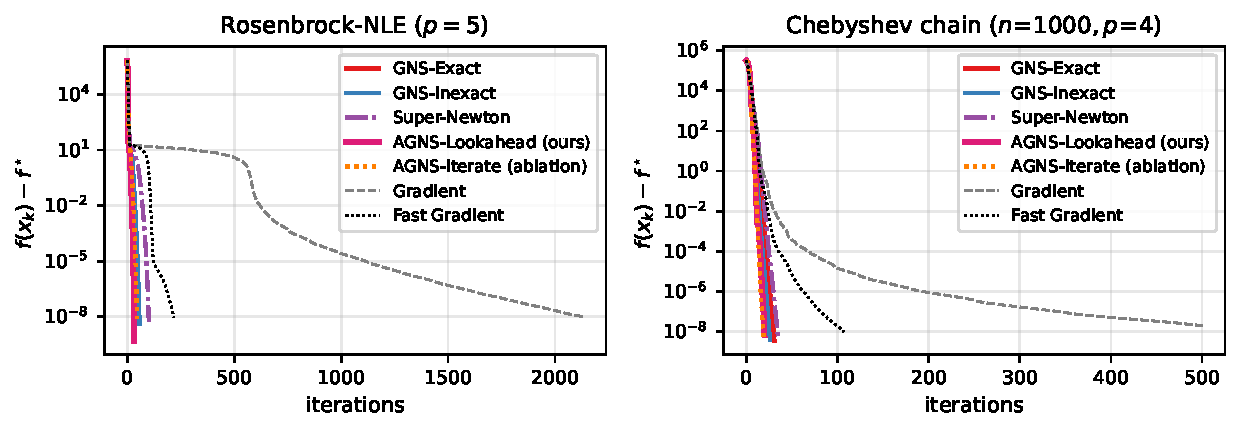
\includegraphics[width=\linewidth]{figs/convergence.pdf}
\caption{\textbf{Convergence on representative non-convex
benchmarks.} \emph{Left}: Rosenbrock-NLE $p=5$ from $x_0=(-2,2)$.
\emph{Right}: Chebyshev polynomial chain, $n=1000, p=4$, $x_0\sim
U[0,1]^n$. Trajectories truncated at the first iterate satisfying
$f(x_k)-f^\star<10^{-8}$; logarithmic $y$-axis.}
\label{fig:convergence}
\end{figure}

\begin{figure}[h]
\centering
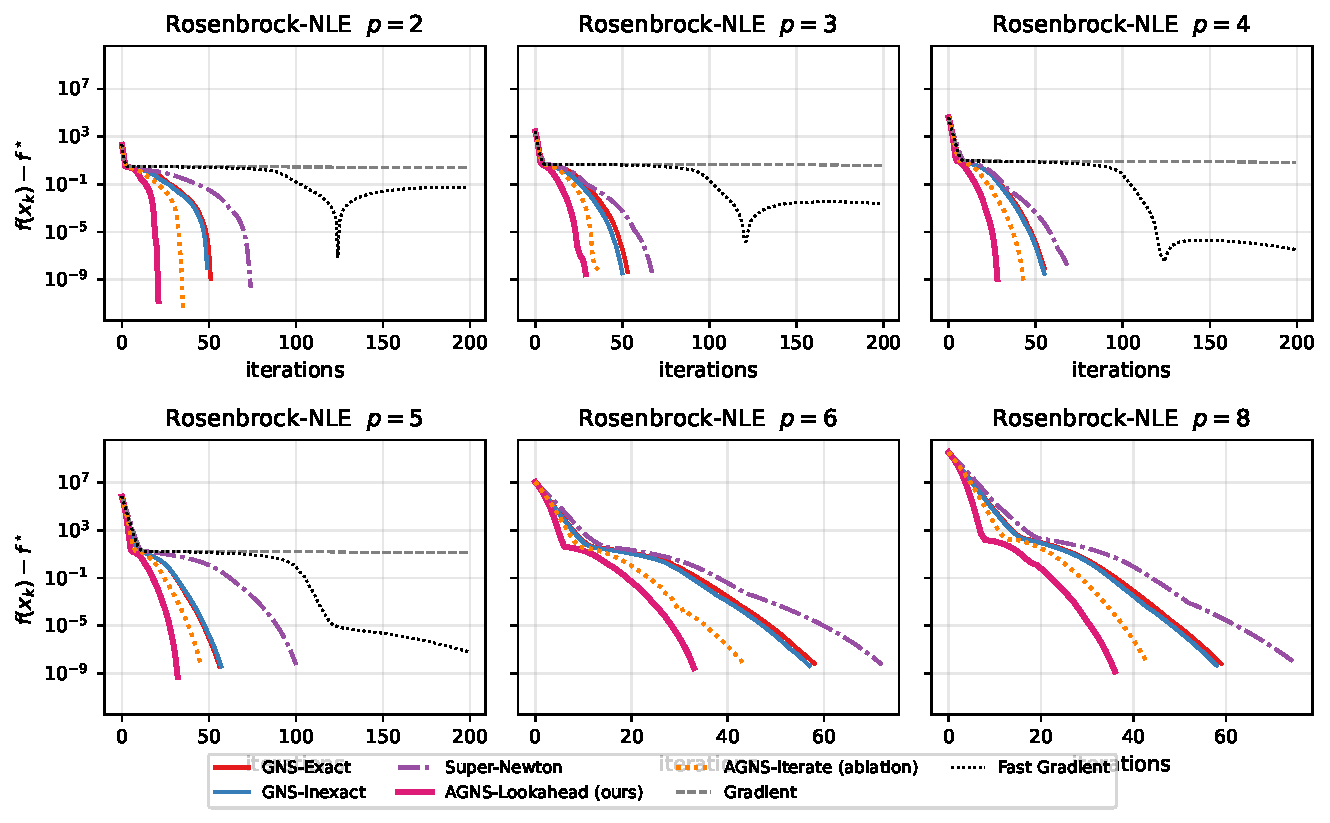
\includegraphics[width=\linewidth]{figs/appendix_psweep.pdf}
\caption{\textbf{Per-iteration convergence on the Rosenbrock-NLE
$p$-sweep.} \AGNS-Lookahead (magenta) is the fastest method on every
panel. Plain gradient and FISTA (gray, black) diverge cleanly at
$p\geq 6$. Horizontal axis truncated at $200$ iterations for
readability.}
\label{fig:psweep}
\end{figure}

\begin{figure}[h]
\centering
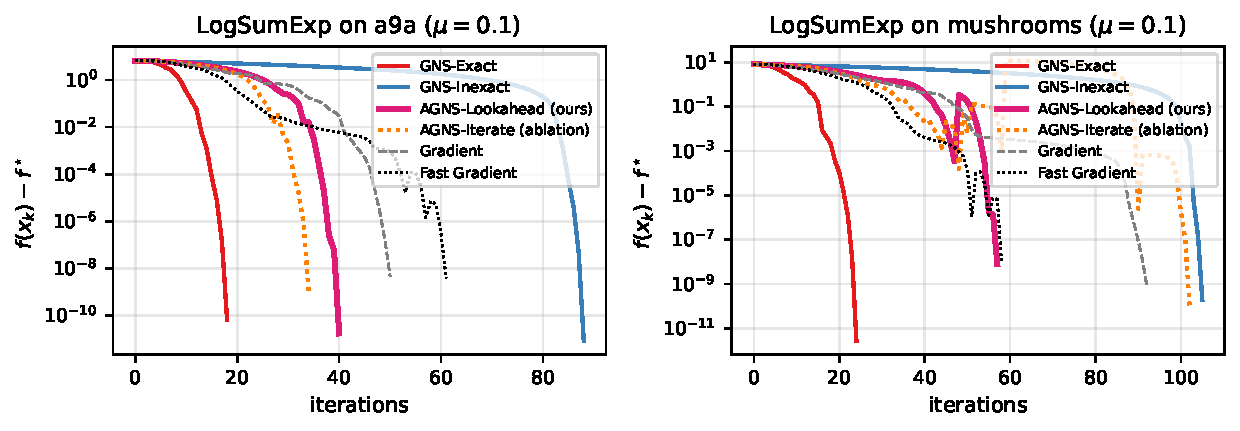
\includegraphics[width=\linewidth]{figs/appendix_logsumexp.pdf}
\caption{\textbf{LogSumExp on real LIBSVM data} (a9a, mushrooms;
$\mu=0.1$). The benchmark where \AGNS\ does \emph{not} accelerate
convergence; \GNS-Exact already attains quadratic local convergence
and reaches the target in $18$ and $24$ iterations respectively,
fewer than \AGNS-Lookahead's $40$ and $57$.}
\label{fig:appendix_lse}
\end{figure}

\begin{figure}[h]
\centering
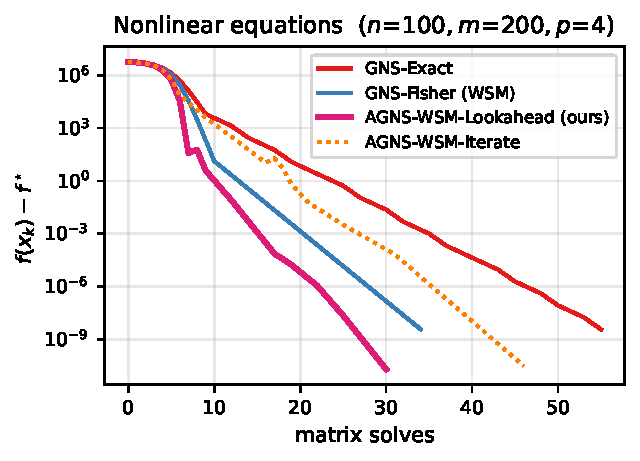
\includegraphics[width=\linewidth]{figs/appendix_matrix_inv.pdf}
\caption{\textbf{Matrix-solve count vs.\ accuracy} on nonlinear
equations ($n=100, m=200, p=4$). \AGNS-WSM-Lookahead needs roughly
half as many solves as \GNS-Exact to reach the same residual.}
\label{fig:matrix_inv}
\end{figure}

\begin{table}[h]
\centering
\small
\caption{Iterations to $\varepsilon=10^{-8}$ on the Rosenbrock-NLE
$p$-sweep ($x_0=(-2,2)$). ``---'' marks
\texttt{line\_search\_diverged}. Best Newton-type method per row in
\textbf{bold}.}
\label{tab:rosenbrock_sweep}
\begin{tabular}{@{}rcccccc@{}}
\toprule
$p$ & GNS-Ex. & GNS-Inex. & Sup.-N. & \AGNS-Look. & Grad. & FastG. \\
\midrule
2 & 51 & 49 & 74  & \textbf{21} & 6852 & 407 \\
3 & 53 & 50 & 67  & \textbf{29} & 4331 & 265 \\
4 & 55 & 55 & 69  & \textbf{28} & 2892 & 238 \\
5 & 56 & 57 & 100 & \textbf{32} & 2132 & 218 \\
6 & 58 & 57 & 72  & \textbf{33} & ---  & --- \\
8 & 59 & 58 & 75  & \textbf{36} & ---  & --- \\
\bottomrule
\end{tabular}
\end{table}

\begin{table}[h]
\centering
\small
\caption{Iterations and wall-clock time to $\varepsilon=10^{-8}$ on
the Chebyshev chain dimension sweep ($p=4$).}
\label{tab:cheb_sweep}
\begin{tabular}{@{}rrrrrl@{}}
\toprule
$n$ & \multicolumn{2}{c}{GNS-Inexact} & \multicolumn{2}{c}{\AGNS-Lookahead} & Speedup \\
\midrule
200  & 22 & 0.073\,s & 16 & 0.057\,s & $1.38\times$ iter, $1.28\times$ time \\
500  & 24 & 1.32\,s  & 18 & 1.12\,s  & $1.33\times$ iter, $1.18\times$ time \\
1000 & 26 & 8.11\,s  & 20 & 6.46\,s  & $1.30\times$ iter, $1.26\times$ time \\
2000 & 27 & 11.97\,s & 19 & 8.26\,s  & $1.42\times$ iter, $1.45\times$ time \\
\bottomrule
\end{tabular}
\end{table}

\begin{table}[h]
\centering
\small
\caption{\textbf{Restart frequency, average $\beta_k$, and maximum
local momentum counter} for \AGNS-Lookahead, measured by an
instrumented run (\texttt{tests/test\_restart\_frequency.py}).
Restart fires on at most $\sim 14\%$ of iterations on every
non-LSE benchmark, far from the every-iteration regime where
Corollary~\ref{cor:fallback} would force degeneracy to \GNS. The momentum
counter $\ell$ reaches $16$ on Rosenbrock-NLE, confirming that long
runs of un-restarted momentum are common in practice.}
\label{tab:restart}
\begin{tabular}{@{}lrrrr@{}}
\toprule
Problem & iters & restart\,\% & avg.\ $\beta_k$ & $\ell_{\max}$ \\
\midrule
Rosenbrock-NLE $p=2$ & 21 & 9.5\,\% & 0.47 & 9 \\
Rosenbrock-NLE $p=4$ & 28 & 7.1\,\% & 0.60 & 16 \\
Rosenbrock-NLE $p=5$ & 32 & 6.2\,\% & 0.55 & 16 \\
Rosenbrock-NLE $p=8$ & 36 & 5.6\,\% & 0.57 & 16 \\
Chebyshev $n=200$  & 16 & 12.5\,\% & 0.36 & 5 \\
Chebyshev $n=500$  & 18 & 11.1\,\% & 0.39 & 6 \\
Chebyshev $n=1000$ & 20 & 10.0\,\% & 0.42 & 6 \\
NLE $p=4$          & 15 & 13.3\,\% & 0.37 & 7 \\
LogSumExp $n{=}m{=}200$ & 22 & 13.6\,\% & 0.43 & 11 \\
\bottomrule
\end{tabular}
\end{table}

\section{Implementation details}
\label{app:algo}

The full \AGNS\ implementation in \texttt{src/methods.py} adds two
guards beyond \Cref{alg:agns}: (i)~if the inner adaptive search
exhausts its budget ($40$ probes) without an accepted step, the trial
point is set to $y_k$ as a safe fallback rather than committed
unconditionally; and (ii)~if $\dnorm{\nabla f(y_k)} < 10^{-8}$, the
Newton step is skipped (we are already at a stationary point near
$y_k$).

For the rank-1 \WSM\ solver, when $p = 2$ the Fisher coefficient
$\alpha = (p-2)\norm{u}^{p-4}$ vanishes and the formula degenerates
to $\Delta = -(\lambda B)^{-1}\nabla f$, i.e.\ a preconditioned
gradient step (the Hessian-approximation contribution is identically
zero for quadratic $f$, which is consistent).

For \GNS-Exact on indefinite Hessians (e.g.\ Chebyshev chain far from
the optimum), Cholesky factorisation initially fails; we catch
\texttt{LinAlgError}, halve $\gamma_k$ to tighten the regularisation,
and retry within the same inner loop. This is mathematically
equivalent to a rejected step.

\end{document}
